\begin{figure}[H]
    \centering
    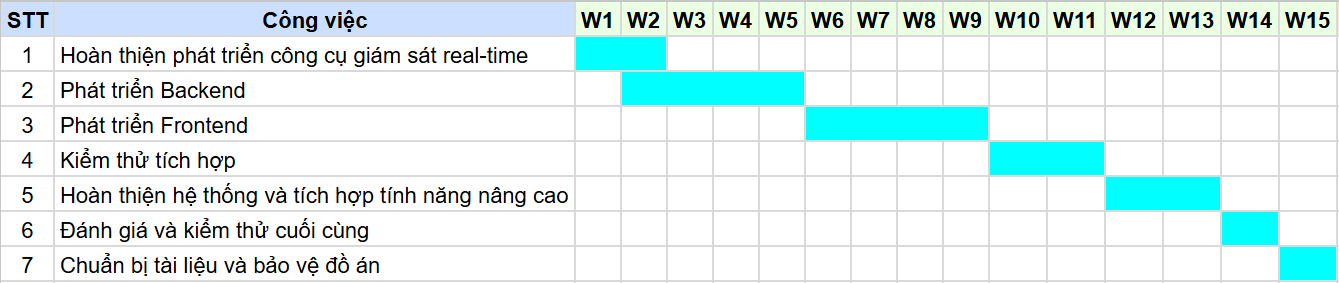
\includegraphics[width=16cm]{Images/GD2-Plan/datn-plan.png}
    \vspace{15pt}
    \caption{Kế hoạch tổng quan cho giai đoạn 2}
\end{figure}

\begin{itemize}

\item\textbf{Task 1: Hoàn thiện phát triển công cụ giám sát real-time (W1-2)}\\
\indent Mục tiêu:
\begin{itemize}
    \item Hoàn thành phát triển công cụ giám sát real-time cài trên máy tính
\end{itemize}
\begin{table}[H]
    \centering
    \begin{tabular}{|p{1cm}|p{8cm}|p{4cm}|}
        \hline
        \textbf{STT} & \textbf{Công việc cụ thể} & \textbf{Thành viên phụ trách} \\
        \hline
        1 & Xác định loại dữ liệu cần thu thập & Hiển   \\
        \hline
        2 & Xác định tần suất thu thập dữ liệu & Khang   \\
        \hline
        3 & Thiết kế công cụ giám sát & Khang  \\
        \hline
        4 & Phát triển công cụ giám sát bằng Python và Kafka & Khang   \\
        \hline
        5 & Kiểm tra lấy dữ liệu từ máy tính bằng công cụ giám sát & Khang, Hiển   \\
        \hline
    \end{tabular}
    
\end{table}

\item\textbf{Task 2: Phát triển Backend (W2-5)}\\
\indent Mục tiêu:
\begin{itemize}
    \item Xây dựng và triển khai các service và API theo thiết kế.
    \item Tích hợp API với cơ sở dữ liệu.
\end{itemize}
\begin{table}[H]
    \centering
    \begin{tabular}{|p{1cm}|p{8cm}|p{4cm}|}
        \hline
        \textbf{STT} & \textbf{Công việc cụ thể} & \textbf{Thành viên phụ trách} \\
        \hline
        1 & Xây dựng hạ tầng cơ bản và tích hợp cơ sở dữ liệu & Khang, Hiển \\
        \hline
        2 & Xây dựng microservice Asset Monitoring Service 
        \begin{itemize}
            \item Tích hợp Kafka Producer
            \item Triển khai Kafka Consumer
        \end{itemize} & Hiển \\
        \hline
        3 & Xây dựng microservice Alert \& Notification Service 
        \begin{itemize}
            \item Xây dựng chức năng và ngưỡng cảnh báo
            \item Tích hợp Kafka để nhận thông tin sự kiện cần gửi thông báo
            \item Tích hợp các phương thức gửi thông báo (email, SMS, push notification...)
            \item Lưu trữ thông tin vào database
        \end{itemize} & Khang\\
        \hline
        4 & Xây dựng User Management Service 
        \begin{itemize}
            \item Quản lý thông tin người dùng và phân quyền
            \item Sử dụng tiêu chuẩn bảo mật OAuth2 để xác thực và phân quyền
            \item Tích hợp JWT (JSON Web Token) hoặc Session-based Authentication
            \item Đảm bảo dữ liệu người dùng được mã hóa (hashed passwords)
        \end{itemize} & Hiển, Tiên \\
        \hline
        5 & Xây dựng Lifecycle Management Service 
        \begin{itemize}
            \item Quản lý vòng đời tài sản (máy tính, phần cứng, phần mềm)
        \end{itemize} & Khang, Hiển, Tiên \\
        \hline
        6 & Xây dựng Data Analysis \& Prediction Service 
        \begin{itemize}
            \item Xây dựng và huấn luyện model phân tích và gợi ý bảo trì tài sản
            \item Tích hợp với các service khác
        \end{itemize} & Khang \\
        \hline
        7 & Xây dựng Inventory Management Service 
        \begin{itemize}
            \item Quản lý thông tin tài sản (máy tính, phần cứng, phần mềm)
            \item Sử dụng UUID để quản lý tài sản
        \end{itemize} & Hiển, Tiên \\
        \hline
        8 & Xây dựng API Gateway 
        \begin{itemize}
            \item Tích hợp xác thực và bảo mật
            \item Rate-limiting, load balancing
        \end{itemize} & Hiển \\
        \hline
        9 & Viết Unit Test cho API & Tiên \\
        \hline
        10 & Kiểm thử các API bằng Postman hoặc Swagger để đảm bảo đúng logic & Tiên \\
        \hline
    \end{tabular}
\end{table}

\item\textbf{Task 3: Phát triển Frontend (W6-9)}\\
\indent Mục tiêu:
\begin{itemize}
    \item Hoàn thiện các màn hình chính đã thiết kế trong UI.
    \item Kết nối giao diện người dùng với API.
\end{itemize}
\begin{table}[H]
    \centering
    \begin{tabular}{|p{1cm}|p{8cm}|p{4cm}|}
        \hline
        \textbf{STT} & \textbf{Công việc cụ thể} & \textbf{Thành viên phụ trách} \\
        \hline
        1 & Tinh chỉnh giao diện Figma & Tiên \\
        \hline
        2 & Xây dựng các Reusable Components & Khang, Hiển, Tiên \\
        \hline
        3 & Sử dụng framework Angular để phát triển các giao diện chính cho các phần 
        \begin{itemize}
            \item Giám sát máy tính
            \item Quản lý máy tính
            \item Quản lý phần cứng
            \item Quản lý phần mềm
            \item Quản lý giấy phép
            \item Quản lý cảnh báo
            \item Quản lý yêu cầu nâng cấp
            \item Quản lý sự cố và bảo trì
            \item Quản lý đơn hàng
            \item Quản lý cấu hình cảnh báo
        \end{itemize} & Khang, Hiển, Tiên \\
        \hline
        4 & Xử lý tính năng giám sát thời gian thực, hiển thị dữ liệu thời gian thực trên giao diện &  Hiển, Tiên \\
        \hline
        5 & Xử lý luồng dữ liệu giữa frontend và backend & Khang \\
        \hline
        6 & Kiểm tra giao diện để đảm bảo hoạt động chính xác & Hiển\\
        \hline
    \end{tabular}
\end{table}

\item\textbf{Task 4: Kiểm thử tích hợp (W10-11)}\\
\indent Mục tiêu:
\begin{itemize}
    \item Đảm bảo hệ thống hoạt động đồng bộ giữa các thành phần (công cụ giám sát, frontend, backend, cơ sở dữ liệu).
\end{itemize}
\begin{table}[H]
    \centering
    \begin{tabular}{|p{1cm}|p{8cm}|p{4cm}|}
        \hline
        \textbf{STT} & \textbf{Công việc cụ thể} & \textbf{Thành viên phụ trách} \\
        \hline
        1 & 
        Chạy các kịch bản kiểm thử tích hợp:
        \begin{itemize}
            \item Tích hợp giữa các microservice
            \item Tích hợp giữa frontend và backend
            \item Tích hợp với cơ sở dữ liệu
        \end{itemize}
        Các loại kiểm thử:
        \begin{itemize}
            \item Kiểm thử chức năng
            \item Kiểm thử tích hợp
            \item Kiểm thử luồng nghiệp vụ (End-to-End Testing)
        \end{itemize} & Hiển, Tiên \\
        \hline
        2 & 
        Kiểm tra các trường hợp lỗi:
        \begin{itemize}
            \item Trường hợp lỗi hệ thống
            \item Trường hợp lỗi dữ liệu
            \item Trường hợp giao diện
        \end{itemize} & Khang \\
        \hline
        3 & 
        Xử lý lỗi phát sinh trong quá trình kiểm thử:
        \begin{itemize}
            \item Ghi nhận lỗi
            \item Phân loại lỗi
            \item Sửa lỗi
            \item Kiểm thử lại
        \end{itemize} & Khang, Hiển, Tiên \\
        \hline
    \end{tabular}
\end{table}

\item\textbf{Task 5: Hoàn thiện hệ thống và tích hợp tính năng nâng cao (W12-13)}\\
\indent Mục tiêu:
\begin{itemize}
    \item Cải tiến và tinh chỉnh giao diện, tính năng.
    \item Đảm bảo hiệu năng và độ ổn định của hệ thống.
    \item Thêm các tính năng nâng cao để cải thiện trải nghiệm người dùng.
\end{itemize}
\begin{table}[H]
    \centering
    \begin{tabular}{|p{1cm}|p{8cm}|p{4cm}|}
        \hline
        \textbf{STT} & \textbf{Công việc cụ thể} & \textbf{Thành viên phụ trách} \\
        \hline
        1 & 
        Chỉnh sửa, tối ưu giao diện người dùng để trực quan và thân thiện hơn. & Tiên \\
        \hline
        2 & 
        Kiểm tra và tối ưu hiệu suất API và cơ sở dữ liệu. & Khang, Hiển \\
        \hline
        3 & 
        Thực hiện và kiểm thử tính năng báo cáo tổng quan:
        \begin{itemize}
            \item Máy tính
            \item Phần cứng
            \item Phần mềm
        \end{itemize} & Khang, Hiển, Tiên \\
        \hline
    \end{tabular}
\end{table}

\item\textbf{Task 6: Đánh giá và kiểm thử cuối cùng (W14)}\\
\indent Mục tiêu:
\begin{itemize}
    \item Đảm bảo hệ thống sẵn sàng triển khai thực tế.
\end{itemize}
\begin{table}[H]
    \centering
    \begin{tabular}{|p{1cm}|p{8cm}|p{4cm}|}
        \hline
        \textbf{STT} & \textbf{Công việc cụ thể} & \textbf{Thành viên phụ trách} \\
        \hline
        1 & Kiểm tra toàn bộ hệ thống với các kịch bản thực tế. & Khang \\
        \hline
        2 & Chạy thử hệ thống trong môi trường doanh nghiệp thực tế và thu thập kết quả. & Hiển \\
        \hline
        3 & Sửa lỗi và cải tiến dựa trên kết quả chạy thử. &  Tiên \\
        \hline
    \end{tabular}
\end{table}

\item\textbf{Task 7: Chuẩn bị tài liệu và bảo vệ đồ án (W15)}\\
\indent Mục tiêu:
\begin{itemize}
    \item Hoàn thiện các tài liệu liên quan đến hệ thống.
    \item Chuẩn bị nội dung bảo vệ đồ án trước hội đồng.
\end{itemize}
\begin{table}[H]
    \centering
    \begin{tabular}{|p{1cm}|p{8cm}|p{4cm}|}
        \hline
        \textbf{STT} & \textbf{Công việc cụ thể} & \textbf{Thành viên phụ trách} \\
        \hline
        1 & Viết tài liệu hướng dẫn sử dụng hệ thống. & Khang, Hiển, Tiên \\
        \hline
        2 & Viết báo cáo đồ án. & Khang, Hiển, Tiên \\
        \hline
        3 & Chuẩn bị bài thuyết trình và luyện tập trả lời câu hỏi từ hội đồng. & Khang, Hiển, Tiên \\
        \hline
    \end{tabular}
\end{table}


\end{itemize}